% author Truong Nhan Nguyen
% created in 16/01/2022

\documentclass[tikz, border=10pt]{standalone}

\usepackage{tikz}
\usetikzlibrary{backgrounds}
\usepackage{xcolor}

\begin{document}
    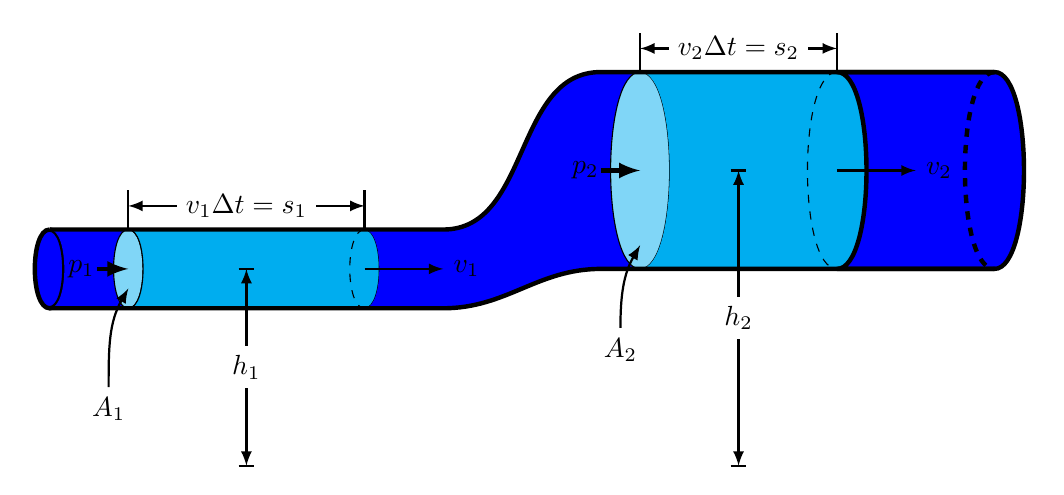
\begin{tikzpicture}
        % \draw[style=help lines] (0, -1) grid (12, 2);
        \draw[ultra thick] 
            (0, 0) -- (5, 0) to[out=0, in=180] (7, 2) -- (12, 2)
            (0, -1) -- (5, -1) to[out=0, in=180] (7, -0.5) -- (12, -0.5);
        \begin{pgfonlayer}{background}[fill opacity=0.8, line join=round]
            \filldraw[fill=blue, ultra thick]
                (0, 0) to[controls=+(180:0.25) and +(180:0.25)] (0, -1)
                to[controls=+(0:0.25) and +(0:0.25)] (0, 0);
            \fill[color=blue] 
                (0, 0) -- (1, 0)
                to[controls=+(180:0.25) and +(180:0.25)] (1, -1)
                -- (0, -1) to[controls=+(0:0.25) and +(0:0.25)] (0, 0); 
            \filldraw[fill=cyan!50]
                (1, 0) to[controls=+(180:0.25) and +(180:0.25)] (1, -1)
                to[controls=+(0:0.25) and +(0:0.25)] (1, 0);
            \filldraw[fill=cyan]
                (1, 0) -- (4, 0)
                to[controls=+(0:0.25) and +(0:0.25)]
                (4, -1) -- (1, -1)
                to[controls=+(0:0.25) and +(0:0.25)] (1, 0);
            \draw[dashed] 
                (4, 0) to [controls=+(180:0.25) and +(180:0.25)] (4, -1);
            \fill[blue]
                (4, 0) -- (5, 0) to[out=0, in=180] (7, 2) -- (7.5, 2)
                to[controls=+(180:0.5) and +(180:0.5)]
                (7.5, -0.5) -- (7, -0.5) to[out=180, in=0] (5, -1)
                -- (4, -1)
                to[controls=+(0:0.25) and +(0:0.25)] (4, 0);
            \filldraw[fill=cyan!50]
                (7.5, 2) to[controls=+(0:0.5) and +(0:0.5)] (7.5, -0.5)
                to[controls=+(180:0.5) and +(180:0.5)] (7.5, 2);
            \fill[cyan]
                (7.5, 2) -- (10, 2)
                to[controls=+(0:0.5) and +(0:0.5)] (10, -0.5)
                -- (7.5, -0.5) to[controls=+(0:0.5) and +(0:0.5)] (7.5, 2);
            \draw[dashed] 
                (10, 2) to[controls=+(180:0.5) and +(180:0.5)] (10, -0.5);
            \filldraw[fill=blue, ultra thick]
                (10, 2) -- (12, 2)
                to[controls=+(0:0.5) and +(0:0.5)] (12, -0.5)
                -- (10, -0.5) to[controls=+(0:0.5) and +(0:0.5)] (10, 2);
            \draw[dashed, ultra thick] 
                (12, 2) to[controls=+(180:0.5) and +(180:0.5)] (12, -0.5);
        \end{pgfonlayer}
        \draw[-latex, thick] (0.75, -2) node[below] {$A_1$} to[out=90, in=240] (1, -0.75);
        \draw[ultra thick, -latex] 
            (0.6, -0.5) node[anchor=east, inner sep=0pt] {$p_1$} -- (1, -0.5);
        \draw[latex-latex, thick] 
            (2.5, -3) -- node[midway, fill=white] {$h_1$} (2.5, -0.5);
        \draw[thick] (2.4, -0.5) -- (2.6, -0.5) (2.4, -3) -- (2.6, -3);
        \draw[thick] (1, 0) -- +(0, 0.5) (4, 0) --+(0, 0.5);
        \draw[latex-latex, thick] 
            (1, 0.3) -- node[midway, fill=white] {$v_1\Delta t = s_1$} (4, 0.3);
        \draw[-latex, thick] (4, -0.5) -- +(1, 0) node[right] {$v_1$};
        \draw[-latex, thick] (7.25, -1.25) node[below] {$A_2$} to[out=90, in=240] (7.5, -0.2);
        \draw[ultra thick, -latex] 
            (7, 0.75) node[anchor=east, inner sep=0pt] {$p_2$} -- (7.5, 0.75);
        \draw[latex-latex, thick] 
            (8.75, 0.75) -- node[midway, fill=white] {$h_2$} (8.75, -3);
        \draw[thick] (8.65, 0.75) -- (8.85, 0.75) (8.65, -3) -- (8.85, -3);
        \draw[thick] (7.5, 2) -- +(0, 0.5) (10, 2) --+(0, 0.5);
        \draw[latex-latex, thick] 
            (7.5, 2.3) -- node[midway, fill=white] {$v_2\Delta t = s_2$} (10, 2.3);
        \draw[-latex, thick] (10, 0.75) -- +(1, 0) node[right] {$v_2$};
    \end{tikzpicture}
\end{document}